\documentclass[12pt]{article}%
\usepackage{algorithm}%
\usepackage{algpseudocode}%
\usepackage{amsmath}%
\usepackage{amssymb}%
\usepackage[backend=bibtex,style=alphabetic,sorting=ynt]{biblatex}
\usepackage{booktabs}%
\usepackage{chemformula}
\usepackage{enumitem}%
\usepackage{geometry}%
\usepackage[symbols,nogroupskip,sort=none]{glossaries-extra}%
\usepackage[colorlinks]{hyperref}%
\usepackage{relsize}%
\usepackage[onehalfspacing]{setspace}%
\usepackage{siunitx}%
\usepackage{tikz}%
\usepackage{xfrac}%

\DeclareSIUnit\Ncm{Nm^3}

\glsxtrnewsymbol[description={Time}]{t}{\ensuremath{t}}%
\glsxtrnewsymbol[description={Space coordinate}]{x}{\ensuremath{x}}%

\glsxtrnewsymbol[description={Time discrete step}]{tau}{\ensuremath{\tau}}%
\glsxtrnewsymbol[description={Space discrete step}]{delta}{\ensuremath{\delta}}%

\glsxtrnewsymbol[description={Specific weight}]{rho}{\ensuremath{\rho}}%
\glsxtrnewsymbol[description={Pressure}]{P}{\ensuremath{P}}%
\glsxtrnewsymbol[description={Temperature}]{T}{\ensuremath{T}}%
\glsxtrnewsymbol[description={Ideal gas constant}]{R}{\ensuremath{R}}%
\glsxtrnewsymbol[description={Molar mass}]{M}{\ensuremath{M}}%

\glsxtrnewsymbol[description={Mass flow rate}]{mdot}{\ensuremath{\dot{m}}}%
\glsxtrnewsymbol[description={Volume flow rate}]{qdot}{\ensuremath{\dot{q}}}%

\glsxtrnewsymbol[description={Enthalpy}]{h}{\ensuremath{h}}%
\glsxtrnewsymbol[description={Heat capacity at constant pressure}]{cp}{\ensuremath{c_{P}}}%
\glsxtrnewsymbol[description={Thermal conductivity}]{k}{\ensuremath{k}}%
\glsxtrnewsymbol[description={Heat transfer coefficient}]{U}{\ensuremath{U}}%
\endinput%
\newcommand{\partialdiff}[2]{\ensuremath{\frac{\partial{#1}}{\partial{#2}}}}

\addbibresource{bibliography.bib}
\usetikzlibrary{shapes,arrows,shapes.geometric}
\geometry{margin=2cm}
\hypersetup{%
	colorlinks  = true,
	linkcolor   = black,
	urlcolor    = black,
	citecolor   = black,
	anchorcolor = black
}

\title{Pre-Sim\\[0.2em]\smaller{}Preprocessing and auxiliary tools for numerical simulation}
\author{W. Dal'Maz Silva}

\begin{document}
\maketitle%
\tableofcontents%
\clearpage%

\section{Module \emph{calphad}}

\subsection{System \ch{Al2O3-CaO}}

System \ch{Al2O3-CaO} is described as provided by \cite{Hallstedt1990}.

%### Liquid
%
%Liquid is described by a 2 sub-lattices ordered ionic melt. The first sub-lattice is occupied by cations $Al^{+3}$ and $Ca^{+2}$. In Hallstedt (1990) the second sublattice contains only $O^{-2}$, being later complemented by $AlO_2^{-1}$ by Mao (2004) as a tentative to improve solubility limits. Thus its stoichiometry is given as $(Al^{+3},Ca^{+2})_P(O^{-2},AlO_2^{-1})_Q$, with the constraint of charge neutrality leading to $P=$ and $Q=$. The following expressions provide the molar Gibbs energy of this phase
%
%$$
%\begin{align*}
%	G_m = &\; y_{Al^{+3}}y_{AlO_2^{-1}}{}^\circ{}G_{Al^{+3}:AlO_2^{-1}} + \\
%	&\; y_{Al^{+3}}y_{O^{-2}}{}^\circ{}G_{Al^{+3}:O^{-2}} + \\
%	&\; y_{Ca^{+2}}y_{AlO_2^{-1}}{}^\circ{}G_{Ca^{+2}:AlO_2^{-1}} + \\
%	&\; y_{Ca^{+2}}y_{O^{-2}}{}^\circ{}G_{Ca^{+2}:O^{-2}} + \\
%	&\; PRT\left(
%	y_{Al^{+3}}\ln{}y_{Al^{+3}} + 
%	y_{Ca^{+2}}\ln{}y_{Ca^{+2}}
%	\right) + \\
%	&\; QRT\left(
%	y_{AlO_2^{-1}}\ln{}y_{AlO_2^{-1}} +
%	y_{O^{-2}}\ln{}y_{O^{-2}}
%	\right) + \\
%	&\; {}^{E}G_m
%\end{align*}
%$$
%
%where
%
%$$
%\begin{align*}
%	{}^{E}G_m = &\; y_{Al^{+3}}y_{Ca^{+2}}y_{AlO_2^{-1}}{}^{0}L + \\
%	&\; y_{Ca^{+2}}y_{AlO_2^{-1}}y_{O^{-2}}\left[
%	{}^{0}L
%	
%	
%	\right]
%\end{align*}
%$$
%
%If we take only early data from Hallstedt (1990), the expressions simplify to the following, with $P=2$ and $Q=2y_{Ca^{+2}}+3y_{Al^{+3}}$
%
%$$
%\begin{align*}
%	G_m = &\; y_{Al^{+3}}{}^\circ{}G_{Al^{+3}:O^{-2}} + \\
%	&\; y_{Ca^{+2}}{}^\circ{}G_{Ca^{+2}:O^{-2}} + \\
%	&\; 2RT\left(
%	y_{Al^{+3}}\ln{}y_{Al^{+3}} + 
%	y_{Ca^{+2}}\ln{}y_{Ca^{+2}}
%	\right) + \\
%	&\; {}^{E}G_m
%\end{align*}
%$$
%
%where
%
%$$
%{}^{E}G_m = y_{Al^{+3}}y_{Ca^{+2}}\left[{}^{0}L + {}^{1}L\left(y_{Al^{+3}} - y_{Ca^{+2}}\right)\right]
%$$

%### $CaO$
%### $3CaO\cdotp{}1Al_2O_3$ ($C_3A_1$)
%### $1CaO\cdotp{}1Al_2O_3$ ($C_1A_1$)
%### $1CaO\cdotp{}2Al_2O_3$ ($C_1A_2$)
%### $1CaO\cdotp{}6Al_2O_3$ ($C_1A_6$)
%### $Al_2O_3$
%### $12CaO\cdotp{}7Al_2O3 (C_{12}A_{7})$

\subsection{System \ch{Al2O3-SiO2}}

\subsection{System \ch{CaO-SiO2}}

System \ch{CaO-SiO2} is described as provided by \cite{Hillert1990}.

%## $CaO$
%## $2CaO\cdotp{}1SiO_2 (C_2S_1)$
%## $3CaO\cdotp{}2SiO_2 (C_3S_2)$
%## $1CaO\cdotp{}1SiO_2 (C_1S_1)$
%## $SiO_2$

\section{Module \emph{heat1d}}

This module aims at solving heat equation for determining temperature profiles across different materials. This is useful as a baseline estimation to check sanity of higher dimensional simulations. In its enthalpy form the equation reads

\begin{equation}
\partialdiff{(\gls{rho}\gls{h})}{\gls{t}} =
\partialdiff{}{\gls{x}}\left(\gls{k}\partialdiff{T}{x}\right)
\label{eq:heat-equation-1d}
\end{equation}

\noindent{}where \gls{rho} is the medium specific mass, \gls{h} the enthalpy, and \gls{k} the thermal conductivity, all evaluated at temperature \gls{T}. Since condensate phases can be approximated to have constant specific weight and from the definition of heat capacity \gls{cp}, the left-hand side time derivative of heat equation can be simplified as

\begin{equation}
\partialdiff{(\gls{rho}\gls{h})}{\gls{t}} =
\gls{rho}\partialdiff{\gls{h}}{\gls{t}} + \partialdiff{\gls{rho}}{\gls{t}}\gls{h} =
\gls{rho}\partialdiff{\gls{h}}{\gls{T}}\partialdiff{\gls{T}}{\gls{t}} =
\gls{rho}\gls{cp}\partialdiff{\gls{T}}{\gls{t}}
\end{equation}

Injecting this result in \eqref{eq:heat-equation-1d} and rearranging terms leads to

\begin{equation}
\partialdiff{\gls{T}}{\gls{t}} =
\frac{1}{\gls{rho}\gls{cp}}
\partialdiff{}{\gls{x}}\left(\gls{k}\partialdiff{T}{x}\right)
\label{eq:heat-equation-1d-simplified}
\end{equation}

In general, for non-constant coefficients \eqref{eq:heat-equation-1d} admits no analytical solutions. Here we proceed with a finite volume method (FVM) discretization. We start the derivation of numerical scheme by integrating the equation in both time and space for one time-step of size \gls{t} over a cell length \gls{delta} as follows

\begin{equation}
\int_{0}^{\gls{delta}}\int_{0}^{\gls{tau}}
\partialdiff{\gls{T}}{\gls{t}} d\gls{t}\,d\gls{x} =
\int_{0}^{\gls{delta}}\int_{0}^{\gls{tau}}
\frac{1}{\gls{rho}\gls{cp}}
\partialdiff{}{\gls{x}}\left(\gls{k}\partialdiff{T}{x}\right) d\gls{t}\,d\gls{x}
\end{equation}

Left-hand side is simply integrated by applying the definition of anti-derivative, while right-hand side has no explicit time dependency and integration is trivially done leading to the multiplication factor 
\gls{tau}.

\begin{equation}
\int_{0}^{\gls{delta}}
\gls{T}^{(\gls{tau})}_{P} - \gls{T}^{(0)}_{P} d\gls{x} =
\int_{0}^{\gls{delta}}
\gls{tau}\frac{1}{\gls{rho}\gls{cp}}
\partialdiff{}{\gls{x}}\left(\gls{k}\partialdiff{T}{x}\right) d\gls{x}
\end{equation}

Figure~\ref{fig:fvm-naming} presents the naming convention for cells in the FVM scheme. Uppercase letters are used to denote cell names. Ghost nodes are also represented, the left-most cell\footnote{Sometimes we call this the upper boundary because it will produce the first roll on the top of matrix produced by the FVM discretization scheme. Conversely, the right side may be called lower boundary.} being called $G$ and right side $H$. Interfaces around reference cell $P$ are represented by the lower case name of the neighbor cell it separates $P$ from, \emph{e.g.} interface $W-P$ is called $w$. It must also be noted that when handling boundary conditions, instead of $W$ or $E$, depending on the side, we make use of $G$ or $H$, lower case letters being used to represent the boundary itself.

\begin{figure}[ht!]
\centering
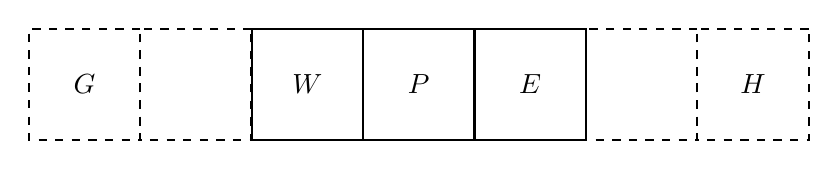
\begin{tikzpicture}[
	auto, thick, node distance=1.415cm, >=triangle 45,
	square/.style={regular polygon,regular polygon sides=4}
	]
	\node [minimum size=2cm,square,draw,name=G,dashed] (G) {$G$};
	\node [minimum size=2cm,square,draw,name=V,right of=G,dashed] (V) {};
	\node [minimum size=2cm,square,draw,name=W,right of=V] (W) {$W$};
	\node [minimum size=2cm,square,draw,name=P,right of=W] (P) {$P$};
	\node [minimum size=2cm,square,draw,name=E,right of=P] (E) {$E$};
	\node [minimum size=2cm,square,draw,name=W,right of=E,dashed] (W) {};
	\node [minimum size=2cm,square,draw,name=H,right of=W,dashed] (H) {$H$};
\end{tikzpicture}
\caption{\label{fig:fvm-naming}Finite volume domain naming convention.}
\end{figure}


Effecting space integration of left-hand side is again trivial and makes cell length \gls{delta} appear in the equation. Anti-derivative of outer space derivative on right hand side is the difference between fluxes over faces $e$ and $w$, as represented by the subscripts.

\begin{equation}
\gls{T}^{(\gls{tau})}_{P} - \gls{T}^{(0)}_{P} =
\frac{\gls{tau}}{\gls{delta}}\frac{1}{\gls{rho}\gls{cp}}
\left[
	\left(\gls{k}\partialdiff{T}{x}\right)_{e} -
	\left(\gls{k}\partialdiff{T}{x}\right)_{w}
\right]
\label{eq:heat-equation-1d-intergrated}
\end{equation}

Computation of the remaining derivatives in \eqref{eq:heat-equation-1d-intergrated} may be subjected to any arbitrary scheme. Here we have chosen to perform this approximation through an upwind scheme as follows

\begin{align}
\left(\gls{k}\partialdiff{T}{x}\right)_{e} &=
\gls{k}_{e}\frac{\gls{T}_{E} - \gls{T}_{P}}{\gls{delta}}\\[6pt]
\left(\gls{k}\partialdiff{T}{x}\right)_{w} &=
\gls{k}_{w}\frac{\gls{T}_{P} - \gls{T}_{W}}{\gls{delta}}
\end{align}

Notice above the introduction of thermal conductivities evaluated at the interfaces. The recommended approach for heat equation is to use an harmonic mean~\cite{Patankar1980} of the values of this coefficient in the neighbor cells, thus $\gls{k}_{j}$ at interface $P-J$ is computed as

\begin{equation}
\gls{k}_{j} = 2\frac{\gls{k}_{P}\gls{k}_{J}}{\gls{k}_{P}+\gls{k}_{J}}
\end{equation}

Next we regroup terms and make a choice regarding time-stepping. Here we adopt a fully implicit approach, thus all temperature and temperature-dependent terms on right-hand side had a superscript denoting their evaluation at the end of time-step $\gls{tau}$, as represented below
 
\begin{equation}
	\gls{T}^{(\gls{tau})}_{P} - \gls{T}^{(0)}_{P} =
	\beta_{P}^{(\gls{tau})}
	\left[
	\gls{k}_{e}^{(\gls{tau})}\gls{T}_{E}^{(\gls{tau})} - (\gls{k}_{e}^{(\gls{tau})} + \gls{k}_{w}^{(\gls{tau})})\gls{T}_{P}^{(\gls{tau})} + \gls{k}_{w}^{(\gls{tau})}\gls{T}_{W}^{(\gls{tau})}
	\right]
\end{equation}

\noindent{}where the coefficient $\beta_{P}$ is given by

\begin{equation}
\beta_{P} = \left(\frac{\gls{tau}}{\gls{delta}^2}\frac{1}{\gls{rho}\gls{cp}}\right)_{P}
\end{equation}

Reordering terms to match Figure~\ref{fig:fvm-naming} and placing all unknowns on left-hand side leads to the general matrix row representation of our numerical scheme given in \eqref{eq:heat-equation-1d-matrix-row}. Notice here that since coefficients are to be computed at unknown temperatures, the solution of the problem is intrinsically iterative. Details of the procedure are explained after boundary conditions are derived for reasons that will become clear later.

\begin{equation}
- \beta_{P}^{(\gls{tau})}\gls{k}_{w}^{(\gls{tau})}\gls{T}_{W}^{(\gls{tau})}
+ \left[
1 + \beta_{P}^{(\gls{tau})}(\gls{k}_{e}^{(\gls{tau})} + \gls{k}_{w}^{(\gls{tau})})
\right]\gls{T}_{P}^{(\gls{tau})}
-\beta_{P}^{(\gls{tau})}\gls{k}_{e}^{(\gls{tau})}\gls{T}_{E}^{(\gls{tau})}
= \gls{T}^{(0)}_{P}
\label{eq:heat-equation-1d-matrix-row}
\end{equation}

Relevant boundary conditions here are varying heat flux Fourier condition and symmetry plane. General Dirichlet and Neumann conditions are ignored in this implementation. Heat convection Fourier boundary condition is stated as

\begin{equation}
-\gls{k}\partialdiff{T}{x} = \gls{U}\left(\gls{T} - \gls{T}_{\infty}\right)
\end{equation}

\noindent{}where \gls{U} is the heat transfer coefficient and $\gls{T}_{\infty}$ environment temperature. This equation can be stated in discrete form for upper boundary as

\begin{equation}
-\gls{k}_{g}^{(\gls{tau})}\frac{\gls{T}_{P}^{(\gls{tau})} - \gls{T}_{G}^{(\gls{tau})}}{\gls{delta}} = \gls{U}\left(\gls{T}_{P}^{(\gls{tau})} - \gls{T}_{\infty}^{(\gls{tau})}\right)
\end{equation}

Since $\gls{k}_{g}$ can be an arbitrary function of temperature and depends of unknown $\gls{T}_{G}$ the above equation is nonlinear and need to be solved through an iterative process. The formal problem of finding ghost node temperatures that respect boundary conditions for upper and lower faces is stated as follows

%TODO I think signs are inversed! At least numerically this doesn't work!

\begin{align}
\gls{T}_{P}^{(\gls{tau})}
- \gls{T}_{G}^{(\gls{tau})}
+ \gamma_{g}^{(\gls{tau})}\left(
	\gls{T}_{\infty}^{(\gls{tau})} - 
	\gls{T}_{P}^{(\gls{tau})}
\right) &= 0
\\[6pt]
-\gls{T}_{P}^{(\gls{tau})} 
+ \gls{T}_{H}^{(\gls{tau})}
- \gamma_{h}^{(\gls{tau})}\left(
	\gls{T}_{\infty}^{(\gls{tau})} - 
	\gls{T}_{P}^{(\gls{tau})}
\right) &= 0
\end{align}

where coefficient $\gamma_{j}$ is defined as

\begin{equation}
	\gamma_{j} = \frac{\gls{U}\gls{delta}}{\gls{k}_{j}}
\end{equation}

Replacing the numerically found $\gls{T}_{G}$ in \eqref{eq:heat-equation-1d-matrix-row} is used to generate first and last rows of numerical scheme matrix. This introduces an additional flux on right-hand side as follows

\begin{align}
\left[
	1 + \beta_{P}^{(\gls{tau})}(\gls{k}_{e}^{(\gls{tau})} + \gls{k}_{g}^{(\gls{tau})})
\right]\gls{T}_{P}^{(\gls{tau})}
-\beta_{P}^{(\gls{tau})}\gls{k}_{e}^{(\gls{tau})}\gls{T}_{E}^{(\gls{tau})}
&= \gls{T}^{(0)}_{P} + 
\beta_{P}^{(\gls{tau})}\gls{k}_{g}^{(\gls{tau})}\gls{T}_{G}^{(\gls{tau})}
\\[6pt]
-\beta_{P}^{(\gls{tau})}\gls{k}_{w}^{(\gls{tau})}\gls{T}_{W}^{(\gls{tau})}
+ \left[
1 + \beta_{P}^{(\gls{tau})}(\gls{k}_{g}^{(\gls{tau})} + \gls{k}_{w}^{(\gls{tau})})
\right]\gls{T}_{P}^{(\gls{tau})}
&= \gls{T}^{(0)}_{P} + 
\beta_{P}^{(\gls{tau})}\gls{k}_{g}^{(\gls{tau})}\gls{T}_{G}^{(\gls{tau})}
\end{align}

A similar approach can be followed to produce first and last rows for symmetry boundary conditions, leading to the next equations

\begin{align}
\left(
1 + \beta_{P}^{(\gls{tau})}\gls{k}_{e}^{(\gls{tau})}
\right)\gls{T}_{P}^{(\gls{tau})}
-\beta_{P}^{(\gls{tau})}\gls{k}_{e}^{(\gls{tau})}\gls{T}_{E}^{(\gls{tau})}
&= \gls{T}^{(0)}_{P}
\\[6pt]
-\beta_{P}^{(\gls{tau})}\gls{k}_{w}^{(\gls{tau})}\gls{T}_{W}^{(\gls{tau})}
+ \left(
1 + \beta_{P}^{(\gls{tau})}\gls{k}_{w}^{(\gls{tau})}
\right)\gls{T}_{P}^{(\gls{tau})}
&= \gls{T}^{(0)}_{P}
\end{align}

It must be emphasized here that use of both convective or symmetry conditions simultaneously is not implied. One may apply convection to one side while using symmetry condition on the other. With all these elements we can now discuss the solution of transient problem. First, if convection condition is used, ghost node temperatures need to be found, but solution $\gls{T}^{(\gls{tau})}$ is unknown. That implies a first estimation of ghost node(s) needs to be done using $\gls{T}^{(0)}$. The same applies to the problem coefficients in left-hand side matrix $\mathbf{M}$ and the vector $\phi$ used to implement convection boundary conditions on right-hand side. Thus the solution of problem can be stated as $\gls{T}^{(\gls{tau})}=\{\mathbf{M}^{(k)}\}^{-1}\left(\gls{T}^{(0)} + \phi^{(k)}\right)$. Algorithm \ref{alg:heat-1d-solution} illustrates time integration with iterative nonlinear solution.

\begin{algorithm}[ht!]
\caption{\label{alg:heat-1d-solution}Iterative solution procedure.}
\begin{algorithmic}
	\State Initialize $\gls{T}^{(0)}$
	
	\For{$\gls{t} \in \vec{\gls{t}}$}
		\Comment{Time loop}
		\State $k \gets 0$
		
		\If{convection}
			\State Find $\gls{T}^{(\gls{tau},k)}_{G}$ using $\gls{T}^{(0)}$
			\State $\phi^{(k)} \gets \phi(\gls{T}^{(\gls{tau},k)}_{G})$
		\Else
			\State $\phi^{(k)} \gets \mathbf{0}$
		\EndIf
		
		\State $\mathbf{M}^{(k)} \gets \mathbf{M}(\gls{T}^{(0)})$
		\State $\gls{T}^{(\gls{tau}, k)} \gets \{\mathbf{M}^{(k)}\}^{-1}\left(\gls{T}^{(0)} + \phi^{(k)}\right)$
			\Comment{Find first approximation of $\gls{T}^{(\gls{tau})}$}
			
		\While{true}
			\Comment{Nonlinear convergence loop}
			\State $k \gets k + 1$
			
			\State $\phi^{(k)} \gets \phi(\gls{T}^{(\gls{tau}, k-1)})$
		
			\If{convection}
				\State Find $\gls{T}^{(\gls{tau},k)}_{G}$ using $\gls{T}^{(\gls{tau}, k-1)}$
				\State $\phi^{(k)} \gets \phi(\gls{T}^{(\gls{tau},k)}_{G})$
			\EndIf
	
			\State $\mathbf{M}^{(k)} \gets \mathbf{M}(\gls{T}^{(\gls{tau}, k-1)})$
			\State $\gls{T}^{(\gls{tau}, k)} \gets \{\mathbf{M}^{(k)}\}^{-1}\left(\gls{T}^{(0)} + \phi^{(k)}\right)$
			
			\If{$\forall \kappa \in \vert{\gls{T}^{(\gls{tau}, k)} - \gls{T}^{(\gls{tau}, k-1)}}\vert, \kappa < \varepsilon$}
				\State $\gls{T}^{(\gls{tau})} \gets \gls{T}^{(\gls{tau}, k)}$
				\State \textbf{break}
			\EndIf
		\EndWhile
		\State $\gls{T}^{(0)} \gets \gls{T}^{(\gls{tau})}$
		\Comment{Reset solution for next time-step}
	\EndFor
\end{algorithmic}
\end{algorithm}

\section{Module \emph{units}}

\subsection{Conversion of \si{\Ncm\per\hour} to \si{\kilo\gram\per\second}}

Assuming ideal gas law, specific weight \gls{rho} can be related to pressure \gls{P}, temperature \gls{T}, and molar mass \gls{M} through ideal gas constant \gls{R} as 

\begin{equation}
\gls{rho} = \dfrac{\gls{P}\gls{M}}{\gls{R}\gls{T}}
\end{equation}

\noindent{}where under normal conditions one set \gls{P} to \SI{101325}{\pascal} and \gls{T} to \SI{288.15}{\kelvin}. The value of \gls{rho} compute this way multiplied by volume flow rate \gls{qdot} provides mass flow rate \gls{mdot}. Conversion of time units is trivial.

\printunsrtglossary[type=symbols,style=long]%

\printbibliography%
\end{document}
